\newthought{Many aspects of the life of a modern human} depend on the theory of \index{signal processing}{signal processing}. Here are a few examples. When you are listening to a digital audio recording of music, displaying an image on your computer, or using a wireless internet connection, you are relying on mathematical concepts that are taught in a basic course on signal processing. These same concepts are encountered when, e.g., solving differential equations, applying deep learning techniques, measuring the gravitational wave signature of colliding neutron stars with a laser interferometer, or making an image of a black hole using a worldwide network of radio telescopes. The theory of \emph{\index{signals and systems}{signals and systems}} is a collection of applied mathematical tools that have important applications in science, technology, and engineering. The term signal processing and the terminology of signal processing have origins in electrical engineering.

\begin{marginfigure}[-4.2cm]
\begin{center}
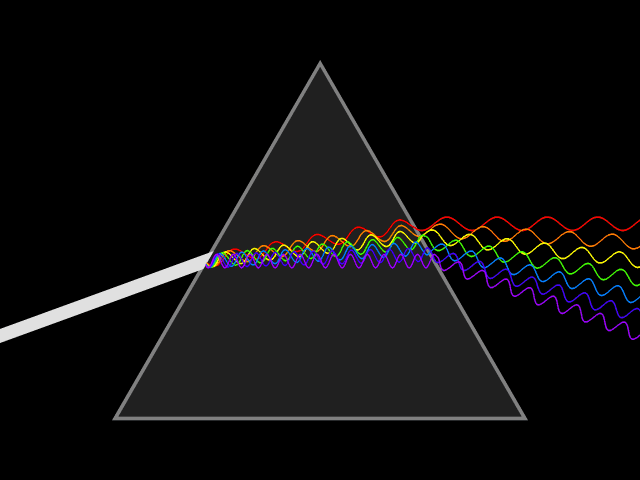
\includegraphics[width=\textwidth]{ch01/figures/prism.png}
\end{center}
\caption{Light can be viewed as a superposition of electromagnetic waves
with different amplitudes, phases, and frequencies. This can be
investigated in practice with the help of a prism or a diffraction
grating. My hope is that after taking this course, you will
metaphorically be able to ``see'' arbitrary signals as a sum of
periodic harmonic functions or \emph{spectral components}.}
\label{fig:prism}
\end{marginfigure}

\newthought{Let's look more closely at the audio example}. When you
listen to a recording of music, you are probably relying on a digital
representation of the acoustic signal that
is \emph{\index{compression}{compressed}}. With the help of signal
processing mathematics, the audio signal is encoded in a special way,
which allows the size of the file to be greatly reduced. This lowers
the minimum internet speed required to stream the audio without
annoying interruptions and allows 10 to 100 times more audio files to
be stored on a digital storage device than without compression.

\index{compression algorithm}{Audio compression algorithms}
often rely on the fact that the \emph{frequency domain}
or \emph{spectral} representation of a signal is far more sparse than
the time domain representation. This means that we can approximate the
original audio signal using a sum of a relatively small number of
periodic sinusoidal signal components. Let's say that the original
audio signal is $x(t)$, which represents air pressure as a function of
time. Using the \index{Fourier series}{Fourier series} we can use the
following type of sum to approximate $x(t)$:
\begin{equation}
x(t) \approx \sum_{n=1}^{N} A_n \sin(\omega_n t + \phi_n) \,\,,
\label{ch01:eq:fourier_ser}
\end{equation}
with each sinusoidal signal only described by three parameters: an
amplitude $A_n \in \mathbb{R}$, a phase $\phi_n \in \mathbb{R}$, and an angular frequency $\omega_n \in \mathbb{R}$.

\begin{marginfigure}
\begin{center}
  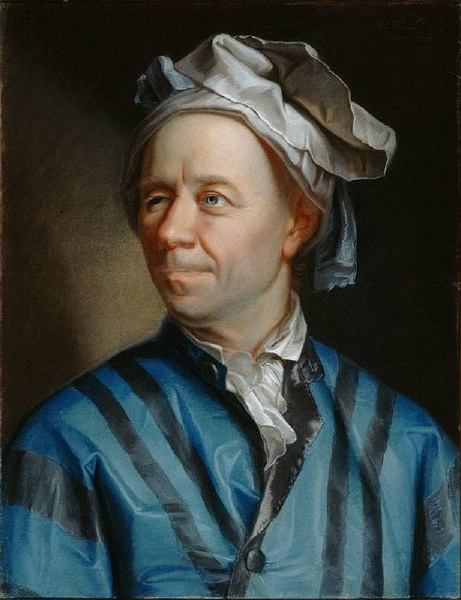
\includegraphics[width=\textwidth]{ch01/figures/euler.jpg}
\end{center}
\caption{Leonhard Euler. Credit: Jakob Handmann (1753)}
\label{fig:euler_pic}
\end{marginfigure}

If the value of $N$ in Equation \ref{ch01:eq:fourier_ser} is
sufficiently small, then the amount of information required to
represent the audio signal as a sum of sinusoids can be significantly
less than what would be required if the signal was just sampled with a
fixed sample spacing and the amplitude of the waveform at each sampled
point would be stored.

Here's an example. Let's say that you want to store 1024 \emph{samples}\sidenote{One sample is a number representing the audio signal amplitude at one instant of time} of
audio signal. With the signal represented using 44100 samples per second,
this would be approximately 0.023 seconds of signal. You'd need to
store 1024 numbers without compression. With 16 bits per sample, this
audio signal would require 16384 bits of storage space. However, if
the signal is sufficiently well represented using $N=10$ sinusoidal
components, you'd only need to store 30 numbers to retain the
information about the phase, amplitude and frequency of each
sinusoidal component. This is only approximately 3\% of the original
data, or 480 bits of storage space at 16 bits per number\sidenote{One
"bit" of information is an answer to a yes or no question. One bit
would allow you to say that a number is either 0 or 1. A two bit
signal would allow you to say that a number is either 0, 1, 2, or 3.}.

Most of the videos, images, and music that you access over the
internet is compressed in this manner. Without spectral compression
techniques, the internet would most likely need to have at least 10
times more capacity than it currently has, in order to be able to
provide us with the same amount of entertainment. For example,
the \index{MP3}{MP3} audio compression standard and
the \index{JPEG}{JPEG} image compression standard both utilize spectral
compression methods.

%This is also the reason why sometimes the audio
%in an online meeting sounds a bit ``robotic'' when you have a very
%poor internet connection -- it is represented with only a small number
%of sinusoidal components. 

\newthought{We often use more general complex valued sinusoidal functions} instead of real valued ones when describing the theory of signal
processing. These are defined as follows:
\begin{equation}
A e^{i\phi }e^{i\omega t} = A[\cos(\omega t+\phi) + i\sin(\omega
t+\phi)] \,\,.
\label{ch01:eq:euler}
\end{equation}
Just like a real-valued sinusoid, the complex sinusoid is also
represented using an amplitude $A \in \mathbb{R}$, phase
$\phi \in \mathbb{R}$, and angular frequency $\omega \in \mathbb{R}$. Note
that the above equation is just an application of Euler's
formula\sidenote[][1cm]{The famous physicist \index{Richard
Feynman}{Richard Feynman} had this to say about \index{Euler's
formula}{Euler's formula}: ``We summarize with this, the most
remarkable formula in mathematics. This is our jewel.'' (Feynman
Lectures on Physics, Vol I). He had clearly benefited greatly from
this formula.}, which is probably the most frequently occurring
equation in signal processing. If you master this equation, you'll
have covered already most of this course!

If you are not familiar with complex algebra,
Equation \ref{ch01:eq:euler} might at first seem intractable. But
don't worry. If you have a hard time grasping the function $A e^{i\phi
}e^{i\omega t}$, just think of it as a periodic function like
$A\cos(\omega t + \phi)$, but with a real and imaginary sinusoidal
component. The reason for using the complex sinusoidal signal instead
of the real valued one is that most of the mathematical calculations
are greatly simplified.

\begin{marginfigure}
\begin{center}
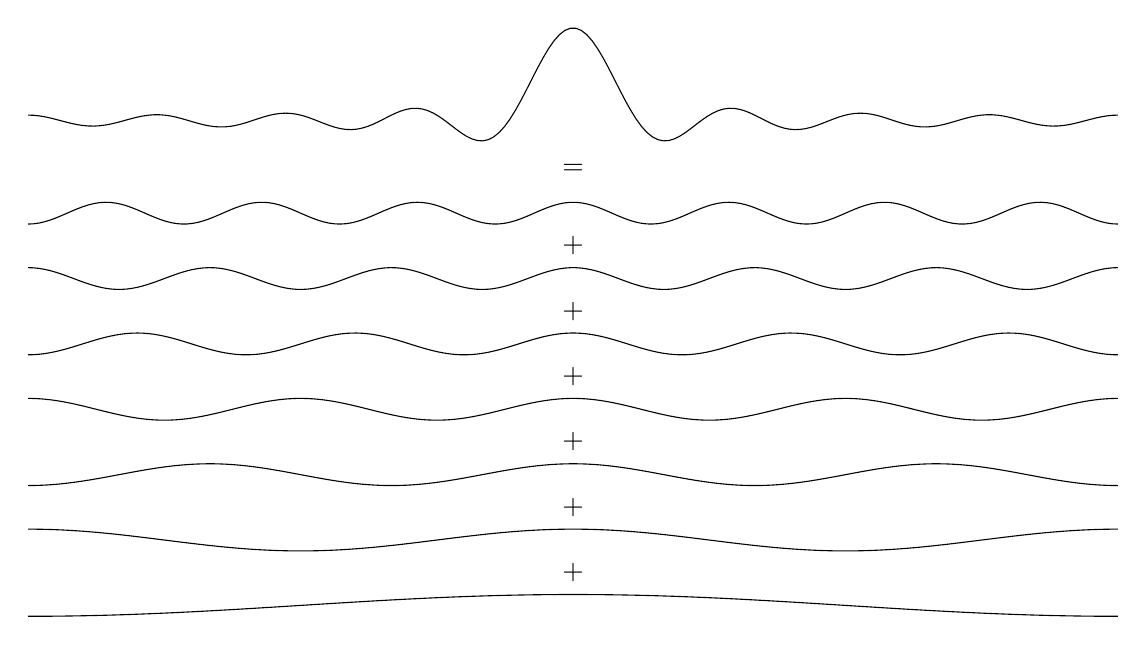
\begin{tikzpicture}
% \begin{pgfinterruptboundingbox}
\begin{axis}[width=1.5\textwidth, height=30em,
%	title={Discrete-time signal},
axis x line=none,
axis y line=none
]
\addplot[domain=-100:100,samples=200] {27+
cos( deg(2*3.1415*0.01*0.5*x))+
cos( deg(2*3.1415*0.01*0.5*2*x) )+
cos( deg(2*3.1415*0.01*0.5*3*x) )+
cos( deg(2*3.1415*0.01*0.5*4*x) )+
cos( deg(2*3.1415*0.01*0.5*5*x) )+
cos( deg(2*3.1415*0.01*0.5*6*x) )+
cos( deg(2*3.1415*0.01*0.5*7*x) )+
cos( deg(2*3.1415*0.01*0.5*8*x) ) };

\node at (axis cs:0,22) {$=$};
\node at (axis cs:0,15) {$+$};
\node at (axis cs:0,9) {$+$};
\node at (axis cs:0,3) {$+$};
\node at (axis cs:0,-3) {$+$};
\node at (axis cs:0,-9) {$+$};
\node at (axis cs:0,-15) {$+$};

\addplot[domain=-100:100,samples=200] {-18+cos( deg(2*3.1415*0.01*0.5*x) ) };
\addplot[domain=-100:100,samples=200] {-12+cos( deg(2*3.1415*0.01*0.5*2*x) ) };
\addplot[domain=-100:100,samples=200] {-6+cos( deg(2*3.1415*0.01*0.5*3*x) ) };
\addplot[domain=-100:100,samples=200] {0+cos( deg(2*3.1415*0.01*0.5*4*x) ) };
\addplot[domain=-100:100,samples=200] {6+cos( deg(2*3.1415*0.01*0.5*5*x) ) };
\addplot[domain=-100:100,samples=200] {12+cos( deg(2*3.1415*0.01*0.5*6*x) ) };
\addplot[domain=-100:100,samples=200] {18+cos( deg(2*3.1415*0.01*0.5*7*x) ) };
\end{axis}
%\end{pgfinterruptboundingbox}
%\draw[use as bounding box] ([xshift=0cm,yshift=0cm]current axis.south west) 
%    rectangle ([xshift=0cm,yshift=0cm]current axis.north east);
\end{tikzpicture}
\end{center}
\caption{Spectral decomposition of a narrow pulse that consists of seven sinusoidal signals.}
\label{fig:dtfig0}
\end{marginfigure}

\begin{marginfigure}
\begin{center}
  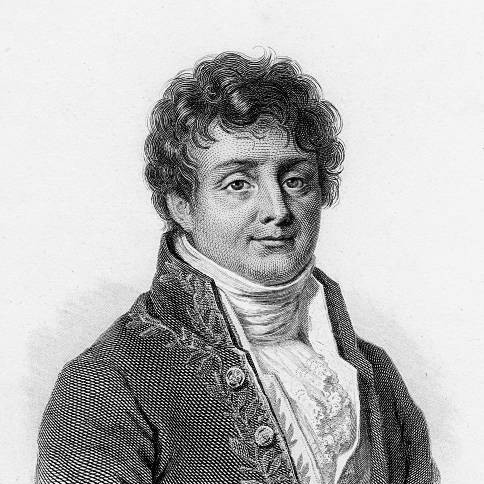
\includegraphics[width=\textwidth]{ch01/figures/fourier_head.jpg}
\end{center}
\caption{Jean-Baptiste Joseph Fourier}
\label{fig:joe_fourier}
\end{marginfigure}

\newthought{A general frequency domain decomposition of signals is known as the \emph{\index{Fourier transform}{Fourier transform}}}. This is just an extended version of the sum of sinusoidal signals given in Equation \ref{ch01:eq:fourier_ser}. The
reverse and forward Fourier transforms allow transforming a signal
between a time domain and a frequency domain representation:
\begin{align}
x(t) &= \frac{1}{2\pi}\int_{-\infty}^{\infty} \hat{x}(\omega) e^{i\omega t} d\omega \\
\hat{x}(\omega) &= \int_{-\infty}^{\infty} x(t) e^{-i\omega t} dt \,\,.
\end{align}
The Fourier transform allows nearly any function to be expressed as an
infinite sum of complex sinusoidal functions, or in other words, an
integral. This is one of the main theoretical foundations of signal
processing. In this equation, the term $x(t)$ is the time domain
representation of the signal, and $\hat{x}(\omega)$ is the frequency
domain representation of the signal. The function $\hat{x}(\omega)$
simply tells you what is the phase $\phi$ and amplitude $A$ of
each spectral component of the signal, assuming that it consists of
infinitely many sinusoidal components.

Figure \ref{fig:dtfig0} shows a sketch of the basic idea behind the
Fourier decomposition of signals. By adding together the seven
individual sinusoidal signals on the bottom of the figure, we obtain
the more pulse-like signal shown on the top of the figure. Conversely,
the pulse-like signal on the top can therefore be decomposed into
seven sinusoidal signals. This is in essence the idea behind the
forward and reverse Fourier transform. Had we continued to sum
together higher and higher frequency sinusoidal signals in the same
manner, we would have ended up with an infinitely narrow spike
$\delta(t)$, which is called the Dirac delta function. This special
function has many important theoretical uses in signal
processing.

The Fourier transform is named after Jean-Baptiste Joseph Fourier, who
is shown in Figure \ref{fig:joe_fourier}. He was the first to come up
with the idea of expressing a function as a sum of sinusoidal signals,
or in other words, spectral components. This occurred in the 1820s
while he was studying heat conduction. Using sinusoidal valued
spectral components to represent the distribution of heat within a
body allowed him to analytically solve the heat equation, because
solving differential equations is relatively straightforward for
sinusoidal functions. Even though this brilliant mathematical
discovery occurred 200 years ago, we are still coming up with new ways
to apply it\sidenote{For example, your smart phone relies on the Fourier
transform in several different ways for enabling transfer of data over
radio waves, and for displaying pictures and videos, and playing audio
files. }. I would say that the ability to divide nearly any function you
encounter into a superposition of simple elementary sinusoidal waves
(the concept of the Fourier transform) is the most useful idea you
will learn from a basic course on signal processing.

If you are not yet completely sure what the equations in this chapter
mean, that is perfectly fine. Learning what the equations are and how
to apply them in practice is the purpose of this course. If you are
already familiar with complex sinusoidal signals and the Fourier
transform, then you may be able to skip much of the introductory
material and spend more time on the application examples.

%% That is it for now. Thank you for listening.
%% The next lecture will discuss how to setup a python programming environment for doing signal processing.
%% The animation that I'm concluding with is a Fourier transform of Jean-Baptiste Joseph Fourier.
%% I have decomposed his figure into two dimensional plane waves, or two dimensional sinusoids.

%% I am showing you what the Fourier series approximation of the picture looks like using a sum of the N largest
%% amplitude spectral components of of the picture of Joseph Fourier looks like. As you can see, when we add more spectral
%% components to the Fourier series approximation, the image quality improves.
%% As you might guess, this is the basic principle behind spectral image compression techniques, such as the JPEG standard.
%% Anyway, see you next time.

%% Here are some other examples of signal processing topics where you
%% will encounter the Fourier transform. You will encounter
%% it when analyzing the properties of filters that modify signals, when
%% applying a filter on a signal, or when searching for solutions of
%% differential equations. The fundamental theorem of discretizing
%% signals, the \emph{Shannon-Nyquist theorem}, relies on the Fourier
%% transform. A two dimensional variant of the Fourier transform is a
%% fundamental part of the theory for making a radio astronomical images
%% using a spatially distributed network of radio telescopes, but it is
%% also often used in image compression.

%Where can one apply the elementary concepts of signal processing
%concepts? Data science, machine learning, differential equations,
%electrical engineering, measurement modeling, telecommunications,
%spectral analysis of measurements, are all examples of application
%areas where basic signal processing concepts are useful.

\if 0
\begin{marginfigure}[1.0cm]
\begin{center}
  \includegraphics[width=\textwidth]{up.jpg}
\end{center}
\caption{Arecibo Observatory radio telescope measurements of the first pulsar ever discovered, CP1919. The vertical axis represents received signal power and the horizontal axis represents time. Successive pulses of the pulsar are shown on each row. The figure is originally from “Radio Observations of the Pulse Profiles and Dispersion Measures of Twelve Pulsars,” by Harold D. Craft, Jr. (September
1970). Signal processing is an important part of practical radio astronomy.}
\end{marginfigure}
\fi



%In many cases, these two categories of signal processing are very
%closely related. For example, the \index{Shannon-Nyquist sampling
%theorem}{Shannon-Nyquist sampling theorem} provides the fundamental
%limits on the information content of a discrete-time signal. It does so by showing
% how a continuous-time signal can be reconstructed perfectly from a
%discrete-time signal, as long as certain conditions on the sample-rate
%and spectral occupancy of the continuous-time signal signal are met.

%The study of signals and systems has evolved significantly over
%time. While many of the fundamental concepts, such as
%the \index{Fourier transform}{Fourier transform} or the Shannon
%sampling theorem, are unchanged and will remain the fundamental
%pillars of signal processing, the exponential increase in the speed of
%general purpose computers has meant that more and more signal
%processing is digital and discrete-time instead of analog.

%Nowadays, digital signal processing is performed mostly with general
%purpose computers and implemented with software, instead of dedicated
%custom digital processing hardware. We will therefore devote much time
%to discrete-time signals and systems and focus on software aspects of
%signal processing in the practical application examples.

%Still, there are always some things that will always remain analog, so
%we cannot completely avoid continuous-time signals. The real world
%itself is continuous, or at least most of us think it is. We therefore
%will cover the theoretical aspects of continuous-time signal
%processing. The continuous-time theory also forms the theoretical
%foundation for much of the discrete-time signal processing.

%However, we will not go into great detail on analog signal
%processing, as this is a topic better suited for a course on circuit
%analysis or radio engineering. We will also not cover any advanced
%continuous-time concepts, such as the Laplace transform, which is a topic perhaps better suited for a course on differential equations.


\begin{marginfigure}%
\begin{center}
\begin{tikzpicture}
\begin{axis}[width=\textwidth,
	xticklabels=\empty,
	yticklabels=\empty,		
	xmin=-1.5,xmax=6,
	axis x line=bottom,
	axis y line=left,
	xlabel={Independent variable $t$},
	xlabel style={below},
	ylabel={Dependent variable $x(t)$},
    xlabel style={ yshift = { 1em } },
    ylabel style={ yshift = { -2.2em } }
]
\addplot[draw=blue,domain=-1:7,samples=150] {(x>0)*exp(-x)};
\end{axis}
\end{tikzpicture}
\end{center}
\caption{Continuous-time signal.}
\label{fig:ctfig_intro}
\end{marginfigure}

\begin{marginfigure}%
\begin{center}
\begin{tikzpicture}
\begin{axis}[width=\textwidth,
%	title={Discrete-time signal},
	xticklabels=\empty,
	yticklabels=\empty,	
	xmin=-1.5,xmax=6,
	axis x line=bottom,
	axis y line=left,
	xlabel={Independent variable $n$},
	xlabel style={below},
	ylabel={Dependent variable $x[n]$},
    xlabel style={ yshift = { 1em } },
    ylabel style={ yshift = { -2.2em } }
]
\addplot+[ycomb,domain=-1:5,samples=15] {(x>0)*exp(-x)};
\end{axis}
\end{tikzpicture}
\end{center}
\caption{Discrete-time signal.}
\label{fig:dtfig_intro}
\end{marginfigure}

\newthought{Signal processing is an interdisciplinary field, where mathematics,
physics, computer science, and engineering intersect}. The theoretical
aspects of signal processing are essentially just applied mathematics,
which often have already been introduced hundreds of years
ago. However, applying the theory to solve real world problems
involves programming or building electrical circuits. This aspect
of signal processing is technology driven, and is continuously
evolving as technology advances. I believe that it is important to be
knowledgeable of both of these aspects in order to successfully apply
signal processing to real world problems.

These lecture notes aim to teach theoretical and applied aspects of signal
processing through mathematical derivations and programming
examples. The mathematics we will use is not rigorous or generalized
in a sense that it would appeal to a mathematician. Similarly, we will
not emphasize aspects of proper software engineering. Instead, the aim
is to provide programming examples that are as simple and as easy to
understand as possible.

My hope is that these notes will take an approach to signal processing
which is appealing to an undergraduate level physics or engineering
student. I do not expect you to have ever encountered a Fourier
transform before, to be familiar with complex algebra, or even be
proficient in programming.

It is natural to divide the topic of signal processing into two main
categories: \emph{\index{continuous-time}{continuous-time}}
and \emph{\index{discrete-time}{discrete-time}}. The former deals with
signals that are continuous functions. The latter deals with signals
that are sequences of numbers, which is more natural for signals that
reside on digital computers and that are used for digital signal
processing. The latter type of signal processing has gained in
importance for quite a long time due to the exponential increase in
computing and storage capacity, which has made it possible to perform
more and more signal processing tasks digitally. The theory for
continuous-time signals lays the theoretical foundation for also the
discrete-time signal processing, so it is still important to teach
this part.

\newthought{This compendium covers} the topics in the syllabus of the
undergraduate signal processing course ``FYS-2006'' held at University
of Troms\o{}. While many other universities will have a separate
``signals and systems'' course that covers continuous-time signals,
and a separate course dedicated to ``digital signal processing'', this
course combines both topics in one course.

These lecture notes are complete in terms of the topics that are
covered in the course ``FYS-2006''. You are not required to obtain any
additional reading material. The reason why I went through the trouble
of typing out these notes is that there currently are no signal
processing textbooks that cover continuous-time and discrete-time
signal processing, and use the Python programming language for
examples. If you wish to deepen your knowledge, there are several
published textbooks that you can use to complement this material. One
book that I recommend is ``Applied Digital Signal Processing: Theory
and Practice'' by D. G. Manolakis and V. K. Ingle.


 %\footnote{For some bizarre reason, the University recently
% changed
%its name to \emph{UiT - The Arctic University of Norway}, where UiT is
%a Norwegian language acronym for University of Troms\o{}. Why there is
%an unexplained acronym in the name of the university, why the word
%university is repeated twice, and why there are two different place
%names is a mystery to many of us working at the university. Some even
%insist on continuing the use of the old name, which further increases
%confusion related to the name of the institution.}.


\newthought{You might be asking yourself: why should I learn about signal processing?} This may be in the minds of, especially those for who have this as a mandatory course, and this is the primary reason that you are attending it. I believe that the elementary concepts taught in a basic course on this topic will provide you with the tools to be a good scientist. You will encounter the mathematical tools introduced in this course throughout science, technology, and engineering, where knowledge of these tools can often be seen as prerequisite background knowledge that allows you to understand more advanced concepts.

Perhaps the most powerful practical tool you will learn during this course is the Fast Fourier Transform (FFT), which is a specific algorithm used to compute a discrete Fourier transformation. It will allow you to perform a wide range of different calculations efficiently, using techniques that are not trivial unless you understand the basic concepts of signal processing. The FFT algorithm can be used e.g., for spectral analysis, evaluation of a convolution operation, to efficiently solve certain types of matrix operations, or to solve differential equations. Any time when processing signals
later on in your life, there is a good chance that you will find the FFT algorithm to be highly useful.

\begin{marginfigure}[1cm]
\begin{center}
  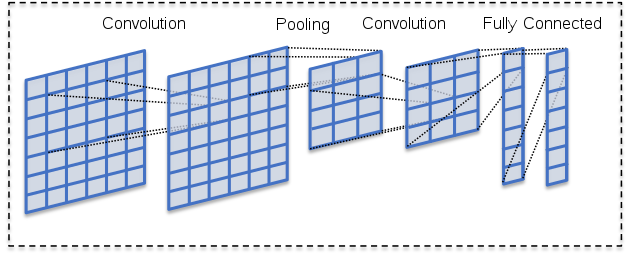
\includegraphics[width=\textwidth]{ch01/figures/cnn.png}
\end{center}
\caption{Simplified diagram of a convolutional neural network, where a convolution operation is one of the fundamental components. Figure adapted from \citep{maier2019gentle}.}
\label{fig:cnn}
\end{marginfigure}

If you go on to work with e.g. machine learning, this course will teach you the concept of convolution, which is a mathematical operation that describes an arbitrary linear time invariant system, and thus plays a major role in signal processing. You may have heard of convolutional neural networks, right? This course will not teach you anything about statistics or neural networks, but it will teach you the concept of a convolution sum, which is often a fundamental
building block of image processing or deep learning
algorithms\cite{maier2019gentle}.